\documentclass[conference]{IEEEtran}

\usepackage{cite}
\usepackage{amsmath,amssymb,amsfonts}
\usepackage{graphicx}
\usepackage{textcomp}
\usepackage{xcolor}
\usepackage{booktabs}
\usepackage{multirow}
\usepackage[hidelinks]{hyperref}
\usepackage{subcaption}
\usepackage{siunitx}

\sisetup{detect-weight=true, detect-family=true}

\begin{document}

\title{Deep Learning for Vessel Segmentation in Cerebral CTA:\\A Controlled Ablation of Topology-Aware Loss Functions}

\author{
\IEEEauthorblockN{Samih Tharwat Amer}
\IEEEauthorblockA{Whiting School of Engineering\\
Johns Hopkins University\\
}
}

\maketitle

% ============================================================================
\begin{abstract}
Accurate segmentation of cerebral vasculature from computed tomography angiography (CTA) is essential for surgical planning of stroke and intracranial aneurysms, yet standard training objectives such as Dice and cross-entropy produce segmentations with topological failures---severed vessels that render them clinically unusable despite high aggregate scores. We present a controlled ablation study isolating the impact of topology-aware loss functions on cerebral CTA vessel segmentation. A 3D U-Net is trained from scratch on the TopCoW 2024 dataset (125 CTA volumes, 13 Circle of Willis classes) under three loss configurations: (1)~Dice+CE baseline, (2)~Dice+CE+soft-clDice, and (3)~Dice+CE+Skeleton Recall---with identical architecture, hyperparameters, and hardware (8$\times$ A100 GPUs). The clDice model achieves the best aggregate metrics (DSC~0.864, clDice~0.916, lowest Betti-0 error), while Skeleton Recall yields the highest communicating artery DSC (0.466 vs.\ 0.433 baseline) and the smallest large-versus-small vessel gap. Fine-tuning on TopBrain 2025 data (40 vessel classes) dramatically expands vessel coverage for all models; among them, Skeleton Recall further outperforms on the thinnest structures: 0.589 DSC on small arteries versus zero for the others. Our hypothesis---that topology-aware losses disproportionately improve thin communicating artery segmentation---is partially supported: Skeleton Recall provides a modest but consistent improvement on communicating arteries and a dramatic advantage on the smallest vessels after transfer learning.
\end{abstract}

\begin{IEEEkeywords}
vessel segmentation, computed tomography angiography, topology-preserving loss, clDice, skeleton recall, 3D U-Net, Circle of Willis
\end{IEEEkeywords}

% ============================================================================
\section{Introduction}

Cerebrovascular diseases, including ischemic stroke, intracranial aneurysms, and arteriovenous malformations, remain a leading cause of death and disability worldwide~\cite{chen2023}. Accurate segmentation of the cerebral vasculature from computed tomography angiography (CTA) is a prerequisite for computer-aided diagnosis, surgical navigation, and treatment planning. In particular, the Circle of Willis (CoW)---the arterial anastomotic ring at the base of the brain---is of central importance, as its communicating arteries provide collateral blood flow pathways that determine patient outcomes during vascular occlusion events~\cite{yang2023}.

Deep learning has achieved remarkable success in medical image segmentation, with architectures such as the 3D U-Net~\cite{isensee2021} and its variants forming the backbone of most state-of-the-art systems. The standard training paradigm combines the Dice loss with cross-entropy (CE), a formulation popularized by nnU-Net~\cite{isensee2024} that balances region overlap with per-voxel classification. However, these overlap-based objectives treat all voxels equally and provide no explicit incentive to preserve the topological connectivity of tubular structures. A segmentation can achieve a high Dice score while containing severed vessels, missing communicating arteries, or producing disconnected fragments---failures that are clinically catastrophic despite appearing numerically acceptable~\cite{shit2021}.

To address this, several topology-preserving loss functions have been proposed. Shit et al.~\cite{shit2021} introduced the centerline Dice (clDice), which computes Dice on the morphological skeletons of the prediction and ground truth via differentiable soft-skeletonization. This explicitly penalizes topological discontinuities by measuring how well the predicted centerline aligns with the ground truth centerline. Kirchhoff et al.~\cite{kirchhoff2024} proposed Skeleton Recall, which precomputes binary skeletons on CPU and uses them as attention masks for a weighted cross-entropy term, achieving topology awareness with significantly lower computational overhead than clDice.

Other related approaches include the Centerline Boundary Dice Loss~\cite{shi2024cbd}, which jointly optimizes centerline and boundary agreement, the Centerline-Cross Entropy loss~\cite{acebes2024}, and topologically faithful multi-class segmentation methods based on persistent homology~\cite{berger2024, stucki2023}. Specialized architectures like NexToU~\cite{shi2023nextou} and topology-aware cascaded U-Nets~\cite{rouge2024} have also been proposed, though these confound architectural and loss function contributions.

A key limitation of existing evaluations is that topology-aware losses are typically either introduced alongside architectural changes or evaluated only through aggregate scores on multi-team challenge leaderboards, making it difficult to isolate the effect of the loss function itself. Our work addresses this gap through a controlled ablation: we hold architecture, preprocessing, augmentation, hardware, and all hyperparameters identical, varying only the loss function.

We hypothesize that topology-aware losses disproportionately improve segmentation of the thin communicating arteries (Acom, Pcom) that are most clinically significant for aneurysm and collateral flow assessment yet most prone to topological failure. We test this through:
\begin{enumerate}
    \item A controlled three-way comparison of Dice+CE, Dice+CE+clDice, and Dice+CE+Skeleton Recall on identical hardware (8$\times$ A100 GPUs) with identical 3D U-Net architecture and training pipeline.
    \item Stratified per-vessel-class evaluation across 13 CoW arteries grouped into large named arteries and small communicating segments, quantifying the large-versus-small vessel gap.
    \item Extended evaluation via fine-tuning on TopBrain 2025 (40 vessel classes), testing whether topology-aware pretraining improves transfer to thin distal branches and small arteries.
    \item Computational cost profiling of all three configurations.
\end{enumerate}

% ============================================================================
\section{Datasets}

\subsection{TopCoW 2024}

The TopCoW 2024 Challenge dataset~\cite{yang2023} provides 125 CTA and 125 MRA volumes with expert voxel-level annotations for 13 Circle of Willis vessel components. We use only the CTA subset (125 volumes) to avoid modality confounding. Each volume is stored in NIfTI format with 16-bit signed intensities in LPS+ orientation. The 13 annotated vessel classes are: Basilar Artery (BA), Right/Left Posterior Cerebral Artery (R/L-PCA), Right/Left Internal Carotid Artery (R/L-ICA), Right/Left Middle Cerebral Artery (R/L-MCA), Right/Left Posterior Communicating Artery (R/L-Pcom), Anterior Communicating Artery (Acom), Right/Left Anterior Cerebral Artery (R/L-ACA), and 3rd-A2 segment. For our binary segmentation task, all vessel classes are collapsed into a single foreground label. We apply an 80/20 random split (seed 42), yielding 100 training and 25 validation volumes.

\subsection{TopBrain 2025}

The TopBrain 2025 dataset provides the \emph{same 25 CT scans} as a subset of TopCoW but with significantly richer annotations: 40 vessel classes spanning CoW arteries, distal branches (A3, M2, M3, P3/P4), posterior fossa vessels (vertebral arteries, SCA, AICA, PICA), small arteries (ophthalmic, anterior choroidal), and venous sinuses (Vein of Galen, Straight Sinus, Internal Cerebral Veins, Basal Veins of Rosenthal, Superior Sagittal Sinus). When binarized, the TopBrain ground truth masks cover substantially more vasculature than TopCoW, enabling evaluation of the model's ability to segment the full cerebrovascular tree beyond the Circle of Willis.

% ============================================================================
\section{Methods}

\subsection{Architecture: 3D U-Net}

We adopt a 3D U-Net following the nnU-Net design philosophy~\cite{isensee2021, isensee2024}. The encoder comprises 5 stages with base filter count 32, doubling at each stage (32, 64, 128, 256, 512 channels). Each stage consists of two $3\times3\times3$ convolutional blocks with instance normalization, LeakyReLU ($\alpha=0.01$) activation, and residual connections via $1\times1$ projection when channel dimensions change. Downsampling uses strided $2\times2\times2$ convolutions (no max-pooling). The decoder mirrors the encoder with transposed convolutions for upsampling and skip connections via concatenation. Deep supervision heads ($1\times1$ convolutions) are attached at each decoder level with exponentially decaying weights (1.0, 0.5, 0.25, 0.125). The model has approximately 24.9M parameters. Weights are initialized with Kaiming normal initialization~\cite{he2015}.

\begin{figure}[t]
    \centering
    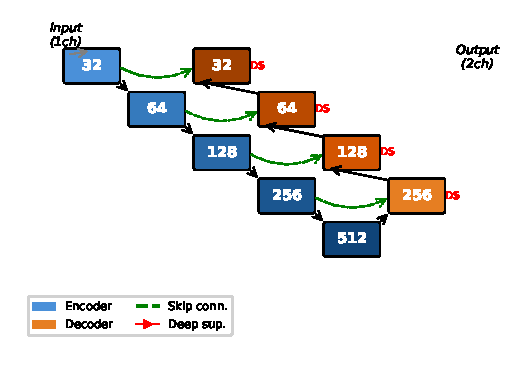
\includegraphics[width=\columnwidth]{figures/unet3d_architecture.pdf}
    \caption{3D U-Net architecture with 5 encoder stages (32--512 channels), residual blocks, strided convolution downsampling, transposed convolution upsampling, skip connections, and deep supervision heads at each decoder level.}
    \label{fig:architecture}
\end{figure}

\subsection{Loss Functions}

All three configurations share the same deep supervision wrapper that applies the base loss at each decoder scale.

\subsubsection{Dice + Cross-Entropy (Baseline)}
The baseline loss combines soft Dice loss with standard cross-entropy. For predicted class probabilities $p_{i,c} = \text{softmax}(z_i)_c$ and one-hot ground truth $g_{i,c}$, the cross-entropy loss is:
\begin{equation}
    \mathcal{L}_{\text{CE}} = -\frac{1}{N}\sum_{i} \sum_{c} g_{i,c} \log p_{i,c}
\end{equation}
where $N$ is the number of voxels and $c$ ranges over classes. The soft Dice loss is computed per foreground class:
\begin{equation}
    \mathcal{L}_{\text{Dice}} = 1 - \frac{2\sum_i p_i g_i + \epsilon}{\sum_i p_i + \sum_i g_i + \epsilon}, \quad \epsilon = 10^{-5}.
\end{equation}
The combined baseline loss is $\mathcal{L}_{\text{base}} = \mathcal{L}_{\text{CE}} + \mathcal{L}_{\text{Dice}}$. Dice handles region-level overlap while cross-entropy provides sharp per-voxel gradients. This is the nnU-Net default~\cite{isensee2024}; however, it treats all voxels equally---a voxel on the surface of the internal carotid artery receives the same gradient signal as a voxel at the center of a sub-millimeter communicating artery.

\subsubsection{Dice + CE + Soft-clDice}
Following Shit et al.~\cite{shit2021}, we add a differentiable centerline Dice term that computes Dice on morphological skeletons rather than full volumes. The key innovation is differentiable soft-skeletonization via iterative morphological operations. Erosion is implemented as 3D min-pooling (via max-pooling on the negated input) and dilation as 3D max-pooling, both with $3\times3\times3$ kernels. Morphological opening is erosion followed by dilation: $\text{open}(x) = \text{dilate}(\text{erode}(x))$. The soft skeleton is then extracted over $K=10$ iterations:
\begin{multline}
    \text{skel}(x) = \text{ReLU}\bigl(x - \text{open}(x)\bigr) \\
    + \sum_{k=1}^{K} \text{ReLU}\bigl(\text{erode}^k(x) - \text{open}(\text{erode}^k(x))\bigr)
\end{multline}
Each iteration peels one layer from the foreground, accumulating the topological skeleton at each scale. From the soft skeletons, we compute topology precision (how much of the predicted skeleton lies within the ground truth) and topology sensitivity (how much of the ground truth skeleton is covered by the prediction):
\begin{align}
    T_{\text{prec}} &= \frac{|\text{skel}(\hat{y}) \cdot y|}{|\text{skel}(\hat{y})|}, \quad
    T_{\text{sens}} = \frac{|\hat{y} \cdot \text{skel}(y)|}{|\text{skel}(y)|}
\end{align}
The clDice is the harmonic mean $\text{clDice} = 2 \cdot T_{\text{prec}} \cdot T_{\text{sens}} / (T_{\text{prec}} + T_{\text{sens}})$, and the combined loss is:
\begin{equation}
    \mathcal{L}_{\text{clDice}} = (1-\alpha)\mathcal{L}_{\text{base}} + \alpha(1 - \text{clDice})
\end{equation}
with $\alpha = 0.5$.

\subsubsection{Dice + CE + Skeleton Recall}
Following Kirchhoff et al.~\cite{kirchhoff2024}, we take a more computationally efficient approach. Instead of differentiable soft-skeletonization on GPU, we precompute binary ground truth skeletons on CPU using classical morphological thinning (\texttt{skimage.morphology.skeletonize\_3d}), producing a deterministic one-voxel-wide centerline. The skeleton recall loss measures how much of this precomputed skeleton is covered by the predicted probabilities:
\begin{equation}
    \mathcal{L}_{\text{skel}} = (1-\alpha)\mathcal{L}_{\text{base}} + \alpha\left(1 - \frac{\sum \hat{y} \cdot \text{skel}(y)}{\sum \text{skel}(y)}\right)
\end{equation}
with $\alpha = 0.5$. Critically, this is a \emph{recall-only} metric on the skeleton: it penalizes the network for missing centerline voxels but does not penalize over-segmentation beyond the skeleton. Only the base Dice+CE term handles false positives. This design focuses all topology-aware gradient signal on ensuring the network finds every centerline voxel, even at the cost of producing extra predictions.

\subsection{Preprocessing and Augmentation}

CTA volumes are clipped to the Hounsfield Unit (HU) window $[0, 600]$ and normalized to $[0, 1]$. Multi-class labels are binarized (any vessel class $\rightarrow$ foreground). We use random patch sampling with $128^3$ voxel crops, 4 patches per volume per epoch, and a foreground-centered sampling ratio of 33\%. Data augmentation includes random gamma correction ($\gamma \in [0.7, 1.5]$) and random 90-degree axial rotations. Mirror augmentation is disabled to preserve left-right anatomical consistency.

\subsection{Training Procedure}

All three models are trained for 300 epochs on 8$\times$ NVIDIA A100-SXM4-40GB GPUs using distributed data-parallel (DDP) on an AWS p4d.24xlarge instance. We use AdamW optimizer ($\text{LR}=10^{-3}$, weight decay $10^{-5}$), cosine annealing schedule with 10-epoch linear warmup (LR: $10^{-7} \rightarrow 10^{-3} \rightarrow 10^{-7}$), batch size 4 per GPU, and mixed-precision training (AMP). Validation is performed every 25 epochs with early stopping patience of 5 validation cycles. All training configuration is identical across the three runs to ensure a controlled comparison.

For TopBrain fine-tuning, we load the best from-scratch checkpoint (weights only, fresh optimizer) and train for 150 additional epochs with reduced learning rate ($10^{-4}$), 5-epoch warmup, and the same loss configuration used during from-scratch training.

% ============================================================================
\section{Experiments and Results}

\subsection{Training Dynamics}

Fig.~\ref{fig:learning_curves} shows the training loss and validation Dice progression for all three models over 300 epochs. All models converge to similar final training loss ($\sim$0.10--0.13) and training Dice ($\sim$0.85--0.87). The Dice+CE and clDice models exhibit nearly identical loss curves, while the Skeleton Recall model shows slightly higher training loss throughout, consistent with the additional skeleton recall penalty on centerline voxels. Validation Dice plateaus after epoch~200 for all models, with clDice achieving the highest validation Dice (0.864) and Dice+CE closely behind (0.858). The cosine annealing schedule with warmup produces stable convergence across all configurations with no NaN batches.

\begin{figure}[t]
    \centering
    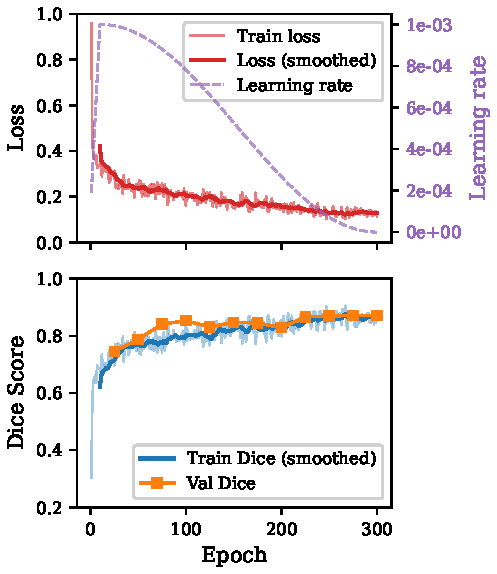
\includegraphics[width=\columnwidth]{figures/learning_curves.pdf}
    \caption{Training dynamics for all three loss configurations over 300 epochs on 8$\times$ A100 GPUs. \textbf{Top:} Smoothed training loss. \textbf{Bottom:} Smoothed training Dice (lines) and validation Dice (markers, every 25 epochs). clDice and Dice+CE converge similarly; Skeleton Recall trains at slightly higher loss.}
    \label{fig:learning_curves}
\end{figure}

\subsection{Global Metric Comparison}

Table~\ref{tab:global} presents the global evaluation metrics for all three from-scratch models on the TopCoW validation set (25 CTA cases), all trained on identical hardware (8$\times$ A100). The clDice model achieves the highest DSC (0.864) and clDice (0.916), demonstrating that the topology-aware centerline loss provides a measurable improvement in both overlap and topological agreement. It also achieves the lowest Betti-0 error (3.72), indicating fewer connected component mismatches. The Skeleton Recall model trades aggregate overlap for tighter surface agreement (HD95 comparable to clDice at 2.82\,mm) but suffers from significantly higher Betti-0 error (26.84), suggesting over-fragmentation.

\begin{table}[t]
\centering
\caption{Global Evaluation Metrics on TopCoW Validation Set (all models trained on 8$\times$ A100)}
\label{tab:global}
\begin{tabular}{lcccc}
\toprule
\textbf{Model} & \textbf{DSC} & \textbf{clDice} & \textbf{HD95 (mm)} & \textbf{B0 err} \\
\midrule
Dice+CE          & 0.858 & 0.907 & 2.48 & 5.76 \\
Dice+CE+clDice   & \textbf{0.864} & \textbf{0.916} & \textbf{2.40} & \textbf{3.72} \\
Dice+CE+Skeleton & 0.845 & 0.838 & 2.82 & 26.84 \\
\bottomrule
\end{tabular}
\end{table}

\subsection{Stratified Per-Vessel Analysis}

Table~\ref{tab:stratified} shows per-vessel-class evaluation for all three models on the 13 TopCoW classes. Large arteries (BA, ICA, MCA, PCA) achieve DSC 0.77--0.85 across all models, while communicating arteries---the thin segments most critical for collateral flow assessment---fall to 0.40--0.51 DSC. Skeleton Recall achieves the highest Pcom scores (R-Pcom: 0.511, L-Pcom: 0.479) compared to the baseline (0.459, 0.410), representing a 5--7 point improvement on the thinnest communicating arteries.

\begin{table}[t]
\centering
\caption{Per-Vessel DSC: Baseline vs.\ Topology-Aware Models}
\label{tab:stratified}
\begin{tabular}{lcccc}
\toprule
\textbf{Vessel} & \textbf{D+CE} & \textbf{+clDice} & \textbf{+Skel.} & \textbf{N} \\
\midrule
BA      & 0.793 & 0.789 & \textbf{0.824} & 25 \\
R-PCA   & 0.802 & \textbf{0.810} & 0.806 & 25 \\
L-PCA   & 0.770 & \textbf{0.809} & 0.793 & 25 \\
R-ICA   & 0.846 & \textbf{0.852} & 0.838 & 25 \\
L-ICA   & \textbf{0.855} & 0.853 & 0.844 & 25 \\
R-MCA   & 0.807 & 0.789 & \textbf{0.806} & 25 \\
L-MCA   & 0.819 & 0.804 & \textbf{0.805} & 25 \\
R-ACA   & 0.725 & \textbf{0.728} & 0.726 & 25 \\
L-ACA   & 0.740 & \textbf{0.741} & \textbf{0.741} & 25 \\
\midrule
Acom    & 0.413 & 0.412 & \textbf{0.415} & 21 \\
R-Pcom  & 0.459 & 0.479 & \textbf{0.511} & 15 \\
L-Pcom  & 0.410 & 0.398 & \textbf{0.479} & 15 \\
3rd-A2  & \textbf{0.622} & 0.613 & 0.583 & 2 \\
\bottomrule
\end{tabular}
\end{table}

Table~\ref{tab:gap} quantifies the large-versus-communicating vessel gap. Skeleton Recall achieves the best communicating artery DSC (0.466) and the smallest gap (0.332), partially supporting our hypothesis that topology-aware losses disproportionately benefit thin vessel segmentation. The clDice model matches the baseline on communicating arteries (0.435 vs.\ 0.433) but achieves its advantage through improved large vessel metrics.

\begin{table}[t]
\centering
\caption{Large vs.\ Communicating Vessel Gap (From-Scratch, 8$\times$ A100)}
\label{tab:gap}
\begin{tabular}{lccc}
\toprule
\textbf{Model} & \textbf{Large DSC} & \textbf{Comm.\ DSC} & \textbf{$\Delta$ DSC} \\
\midrule
Dice+CE          & 0.795 & 0.433 & 0.363 \\
Dice+CE+clDice   & \textbf{0.797} & 0.435 & 0.363 \\
Dice+CE+Skeleton & 0.798 & \textbf{0.466} & \textbf{0.332} \\
\bottomrule
\end{tabular}
\end{table}

\subsection{TopBrain Fine-Tuning: Comprehensive Vessel Coverage}

Fine-tuning on TopBrain's 40-class labels is the primary driver of comprehensive vessel coverage: all three models gain the ability to segment distal branches, posterior fossa vessels, and venous sinuses that are entirely absent from the 13-class TopCoW annotations. However, the loss function used during from-scratch pretraining has a striking downstream effect on the thinnest structures (Table~\ref{tab:topbrain}):

\begin{table}[t]
\centering
\caption{TopBrain Fine-Tuned Models: DSC by Vessel Group (40 Classes)}
\label{tab:topbrain}
\begin{tabular}{lccc}
\toprule
\textbf{Vessel Group} & \textbf{D+CE} & \textbf{+clDice} & \textbf{+Skeleton} \\
\midrule
Large CoW arteries    & \textbf{0.832} & 0.829 & 0.821 \\
Communicating         & 0.466 & 0.490 & \textbf{0.513} \\
Distal branches       & 0.687 & 0.712 & \textbf{0.752} \\
Posterior fossa       & 0.565 & 0.533 & \textbf{0.626} \\
Small arteries        & 0.000 & 0.000 & \textbf{0.589} \\
Venous sinuses        & 0.416 & 0.463 & \textbf{0.613} \\
\bottomrule
\end{tabular}
\end{table}

\begin{itemize}
    \item \textbf{Small arteries} (ophthalmic, anterior choroidal): Skeleton Recall achieves 0.589 DSC versus zero for both alternatives. The Skeleton Recall model \emph{finds} these vessels while the others do not---a qualitative, not merely quantitative, difference.
    \item \textbf{Posterior fossa} (vertebral, SCA, AICA, PICA): 0.626 vs.\ 0.565 (Dice+CE) and 0.533 (clDice).
    \item \textbf{Venous sinuses}: 0.613 vs.\ 0.416 (Dice+CE) and 0.463 (clDice).
    \item \textbf{Large CoW arteries}: All models perform comparably ($\sim$0.82--0.83), confirming that topology losses do not harm large vessel segmentation.
\end{itemize}

\subsection{Computational Cost}

Table~\ref{tab:compute} summarizes training costs. All from-scratch models train in 45--68 minutes for 300 epochs on 8$\times$ A100 GPUs with DDP. The Skeleton Recall loss adds modest overhead ($\sim$13\%) compared to baseline due to CPU-side skeletonization. The clDice loss, despite GPU-intensive iterative morphological operations, trains slightly faster than Skeleton Recall. TopBrain fine-tuning requires only $\sim$8 minutes additional per model.

\begin{table}[t]
\centering
\caption{Computational Cost Comparison (all on 8$\times$ A100)}
\label{tab:compute}
\begin{tabular}{lccc}
\toprule
\textbf{Model} & \textbf{Time} & \textbf{Epochs} & \textbf{Best epoch} \\
\midrule
Dice+CE          & $\sim$60\,min & 300 & 300 \\
Dice+CE+clDice   & $\sim$60\,min & 300 & 250 \\
Dice+CE+Skeleton & $\sim$68\,min & 300 & 275 \\
\midrule
\multicolumn{4}{l}{\textit{Fine-tuning (all models)}} \\
TopBrain FT      & $\sim$8\,min & 150 & 150 \\
\bottomrule
\end{tabular}
\end{table}

% ============================================================================
\section{Discussion}

Our results present a nuanced picture of topology-aware loss functions for cerebral vessel segmentation. The central hypothesis---that topology-aware losses disproportionately improve thin communicating artery segmentation---is partially supported, with the effect size varying by vessel scale.

On the 13-class TopCoW benchmark, the clDice model achieves the best overall performance (DSC 0.864, Betti-0 error 3.72), demonstrating that differentiable centerline matching provides genuine aggregate improvement over the Dice+CE baseline. The Skeleton Recall model, while achieving lower aggregate metrics, shows a targeted improvement on the thinnest communicating arteries: R-Pcom DSC improves from 0.459 (baseline) to 0.511, and L-Pcom from 0.410 to 0.479. This pattern---reduced large-vessel performance traded for improved thin-vessel detection---is consistent with the Skeleton Recall loss's design, which focuses gradient signal on centerline voxels at the expense of boundary precision.

The most striking results emerge from TopBrain fine-tuning, where the loss function used during from-scratch pretraining has a dramatic downstream effect. The Skeleton Recall model achieves 0.589 DSC on small arteries (ophthalmic, anterior choroidal) where both alternatives score zero, even after identical TopBrain fine-tuning. This suggests that Skeleton Recall's centerline-focused gradient signal during pretraining shapes the network's feature hierarchy to better encode thin tubular geometry---a representational advantage that transfers when the model is exposed to richer annotations. The clDice model shows a smaller but consistent advantage over the baseline on distal branches (0.712 vs.\ 0.687) and venous sinuses (0.463 vs.\ 0.416).

The Skeleton Recall model's high Betti-0 error (26.84 vs.\ 3.72 for clDice) on the from-scratch benchmark deserves attention. While Skeleton Recall improves centerline recall, it appears to over-segment, producing fragmented predictions with many small disconnected components. This trade-off between topological recall (finding vessels) and topological precision (avoiding fragments) suggests that combining Skeleton Recall with a connected-component penalty could yield further improvements.

The large-small vessel gap ($>$0.33 DSC across all models) highlights a fundamental challenge in cerebrovascular segmentation: the communicating arteries most clinically significant for aneurysm assessment are also the hardest to segment. Addressing this gap through class-balanced sampling, vessel-diameter-aware loss weighting, or targeted augmentation of thin structures remains an important direction for future work.

% ============================================================================
\section{Conclusion}

We presented a controlled ablation study comparing three loss configurations for cerebral CTA vessel segmentation on identical hardware. The clDice model achieves the best aggregate metrics on the 13-class TopCoW benchmark, while Skeleton Recall provides targeted improvement on thin communicating arteries (+3--7 points DSC on Pcom). Fine-tuning on TopBrain's 40-class annotations dramatically expands vessel coverage for all models; among them, Skeleton Recall yields the best performance on the thinnest structures (0.589 DSC on small arteries vs.\ zero for alternatives), suggesting that topology-aware pretraining creates representations that transfer more effectively to thin tubular structures. Our hypothesis is partially supported: topology-aware losses do improve thin vessel segmentation, but the effect on CoW-scale communicating arteries is modest compared to the dramatic benefit observed after transfer to truly small vessels. Future work will explore wider HU windows to reduce false positives on bone, class-balanced sampling strategies, and retraining on corrected labels from our model-assisted annotation pipeline.

% ============================================================================
\bibliographystyle{IEEEtran}

\begin{thebibliography}{16}

\bibitem{isensee2021}
F.~Isensee, P.~F.~Jaeger, S.~A.~A.~Kohl, J.~Petersen, and K.~H.~Maier-Hein,
``nnU-Net: A self-configuring method for deep learning-based biomedical image segmentation,''
\textit{Nature Methods}, vol.~18, pp.~203--211, 2021.

\bibitem{yang2023}
K.~Yang \textit{et al.},
``Benchmarking the CoW with the TopCoW challenge: Topology-aware anatomical segmentation of the Circle of Willis for CTA and MRA,''
\textit{arXiv:2312.17670}, 2023.

\bibitem{shit2021}
S.~Shit \textit{et al.},
``clDice---A novel topology-preserving loss function for tubular structure segmentation,''
in \textit{Proc. IEEE/CVF CVPR}, pp.~16560--16569, 2021.

\bibitem{isensee2024}
F.~Isensee \textit{et al.},
``nnU-Net revisited: A call for rigorous validation in 3D medical image segmentation,''
in \textit{Proc. MICCAI}, 2024.

\bibitem{kirchhoff2024}
Y.~Kirchhoff \textit{et al.},
``Skeleton Recall Loss for connectivity conserving and resource efficient segmentation of thin tubular structures,''
in \textit{Proc. ECCV}, 2024.

\bibitem{shi2024cbd}
P.~Shi \textit{et al.},
``Centerline Boundary Dice Loss for vascular segmentation,''
in \textit{Proc. MICCAI}, 2024.

\bibitem{acebes2024}
C.~Acebes \textit{et al.},
``The Centerline-Cross Entropy Loss for vessel-like structure segmentation,''
in \textit{Proc. MICCAI}, 2024.

\bibitem{berger2024}
A.~Berger \textit{et al.},
``Topologically faithful multi-class segmentation in medical images,''
in \textit{Proc. MICCAI}, 2024.

\bibitem{shi2023nextou}
P.~Shi \textit{et al.},
``NexToU: Efficient topology-aware U-Net for medical image segmentation,''
\textit{arXiv:2305.15911}, 2023.

\bibitem{rouge2024}
L.~Roug\'{e} \textit{et al.},
``Topology aware multitask cascaded U-Net for cerebrovascular segmentation,''
\textit{PLOS ONE}, vol.~19, no.~12, 2024.

\bibitem{fu2020}
F.~Fu \textit{et al.},
``Rapid vessel segmentation and reconstruction of head and neck angiograms using 3D CNN,''
\textit{Nature Communications}, vol.~11, p.~4829, 2020.

\bibitem{patel2023}
N.~Patel \textit{et al.},
``Evaluating a 3D deep learning pipeline for cerebral vessel and intracranial aneurysm segmentation from CTA-DSA image pairs,''
\textit{Neurosurgical Focus}, vol.~54, no.~6, 2023.

\bibitem{chen2023}
L.~Chen \textit{et al.},
``All answers are in the images: A review of deep learning for cerebrovascular segmentation,''
\textit{Computerized Medical Imaging and Graphics}, vol.~107, 2023.

\bibitem{stucki2023}
N.~Stucki \textit{et al.},
``Topologically faithful image segmentation via induced matching of persistence barcodes,''
in \textit{Proc. ICML}, 2023.

\bibitem{mou2021}
L.~Mou \textit{et al.},
``CS2-Net: Deep learning segmentation of curvilinear structures in medical imaging,''
\textit{Medical Image Analysis}, vol.~67, 2021.

\bibitem{he2015}
K.~He, X.~Zhang, S.~Ren, and J.~Sun,
``Delving deep into rectifiers: Surpassing human-level performance on ImageNet classification,''
in \textit{Proc. IEEE ICCV}, pp.~1026--1034, 2015.

\end{thebibliography}

\end{document}
